\documentclass[11pt, a4paper]{article}

\usepackage{tikz}
\usetikzlibrary{datavisualization}
\usetikzlibrary{datavisualization.formats.functions}
\usetikzlibrary{shapes}
\usepackage{multirow}
\usepackage{commath}
\usepackage{amsmath}
\usepackage{booktabs}
\usepackage{placeins}

\begin{document}

\title{DECISION TREES}
\date{}
\maketitle

One of the most widely used and effective learning method to approximate discrete valued target functions.

\section{Algorithm}

\begin{enumerate}
	\item Use a heuristic to select an attribute for the root node.
	\item Create branches for each possible value of the attribute.
	\item Split the instances having a particular attribute value to the corresponding branch's node.
	\item Repeat recursively for each branch and stop recursion for a branch if all instances have the same class.
\end{enumerate}

\section{Attribute Selection Heuristic}

Prefer attribute which splits the data into purest successor nodes. Entropy is such a measure of disorder. For a set of items belonging to two classes positive and negative, 

\begin{align*}
	\mathbf{E}(p, n) = -\frac{p}{p + n} \times log_2(\frac{p}{p + n}) -\frac{n}{p + n} \times log_2(\frac{n}{p + n}) 
\end{align*}

\begin{figure}
	\centering
	\resizebox{20em}{10em}{
		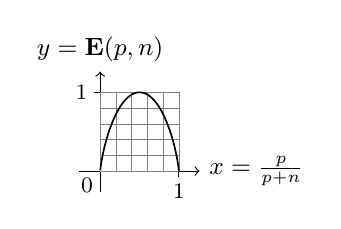
\begin{tikzpicture}
			\draw[step = 0.2 cm, gray, very thin] (0, 0) grid ( 1, 1);
			\datavisualization [school book axes,
				visualize as smooth line,
				y axis={label={$y=\mathbf{E}(p, n)$}},
			x axis={label={$x=\frac{p}{p + n}$}} ]
			
			data [format=function] {
				var x : interval [0.001:1] samples 100;
				func y = -\value x * log2(\value x) - (1 -\value x) * log2(1 -\value x);
			};
		\end{tikzpicture}
	}
	\caption{Entropy in two class distribution}
\end{figure}

Generally for $n$ classes,

\begin{align*}
	\mathbf{E}(S) = \mathbf{E}(p_1,\ p2,\ ...,\ p_n) = -\sum_{i=1}^{n} p_i \times log_2(p_i) \\
	                                                                                         \\
\end{align*}

Entropy only calculates the quality of a single split sub-set. To calculate the quality of the entire split over the attribute $A$, 

\begin{align*}
	\mathbf{Gain}(S, A) = \mathbf{E}(S) -\sum_i \frac{\abs{S_i}}{\abs{S}} \times \mathbf{E}(S_i) 
\end{align*}

The attribute that maximizes the information gain is selected.

\section{Example}

\begin{table}[h!]
	\centering
	\caption{Training data}
	\label{tab:table1}
	\begin{tabular}{c|cccc|c}
		\toprule
		\textbf{Sr.} & \textbf{Outlook} & \textbf{Temperature} & \textbf{Humidity} & \textbf{Windy} & \textbf{PlayGolf} \\
		\midrule
		1            & Sunny            & Hot                  & High              & False          & No                \\
		2            & Sunny            & Hot                  & High              & True           & No                \\
		3            & Overcast         & Hot                  & High              & False          & Yes               \\
		4            & Rainy            & Cool                 & Normal            & False          & Yes               \\
		5            & Overcast         & Cool                 & Normal            & True           & Yes               \\
		6            & Sunny            & Mild                 & High              & False          & No                \\
		7            & Sunny            & Cool                 & Normal            & False          & Yes               \\
		8            & Rainy            & Mild                 & Normal            & False          & Yes               \\
		9            & Sunny            & Mild                 & Normal            & True           & Yes               \\
		10           & Overcast         & Mild                 & High              & True           & Yes               \\
		11           & Overcast         & Hot                  & Normal            & False          & Yes               \\
		12           & Rainy            & Mild                 & High              & True           & No                \\
		13           & Rainy            & Cool                 & Normal            & True           & No                \\
		14           & Rainy            & Mild                 & High              & False          & Yes               \\
		\bottomrule
	\end{tabular}
\end{table}
~\\
All four attributes - \textbf{Outlook}, \textbf{Temperature}, \textbf{Humidity} and \textbf{Windy} are candidates for evaluation to choose the best splitting attribute.
~\\

\begin{align*}
	\textbf{E}(S) & = -\frac{9}{14}\times log2(\frac{9}{14}) - \frac{5}{14} \times log2(\frac{5}{14}) \\
	              & = 0.940\ \textbf{bits}                                                            
\end{align*}

\subsection*{Outlook Gain}

\FloatBarrier
\begin{table}[h]
	\centering
	\label{tab:table2}
	\begin{tabular}{c|cc|c|c}
		\toprule
		\textbf{Outlook}        & \textbf{Yes} & \textbf{No} & \textbf{Split\ Entropy}                                                              & \textbf{Split Weight} \\
		\midrule
		\rule{0pt}{1ex}Rainy    & 3            & 2           & $-\frac{3}{5}\times log_2(\frac{3}{5})-\frac{2}{5}\times log_2(\frac{2}{5}) = 0.971$ & $\frac{5}{14}$        \\ [1ex]
		
		\rule{0pt}{1ex}Overcast & 4            & 0           & $-\frac{4}{4}\times log_2(\frac{4}{4})-\frac{0}{4}\times log_2(\frac{0}{4}) = 0$     & $\frac{4}{14}$        \\ [1ex]
		
		\rule{0pt}{1ex}Sunny    & 2            & 3           & $-\frac{2}{5}\times log_2(\frac{2}{5})-\frac{3}{5}\times log_2(\frac{3}{5}) = 0.971$ & $\frac{5}{14}$        \\ [1ex]
		
	\end{tabular}
\end{table}

\begin{align*}
	\textbf{Gain}(S, Outlook) & = \mathbf{E}(S) - (\frac{5}{14}\times 0.971 + \frac{4}{14} \times 0 + \frac{5}{14} \times 0.971) \\   
	                          & = 0.940 - 0.694                                                                                  \\
	                          & = 0.246\ \textbf{bits}                                                                           \\  
\end{align*}

\subsection*{Temperature Gain}

\FloatBarrier
\begin{table}[h]
	\centering
	\label{tab:table3}
	\begin{tabular}{c|cc|c|c}
		\toprule
		\textbf{Temperature} & \textbf{Yes} & \textbf{No} & \textbf{Split\ Entropy}                                                              & \textbf{Split Weight} \\
		\midrule
		\rule{0pt}{1ex}Cool  & 3            & 1           & $-\frac{3}{4}\times log_2(\frac{3}{4})-\frac{1}{4}\times log_2(\frac{1}{4}) = 0.811$ & $\frac{4}{14}$        \\ [1ex]
		
		\rule{0pt}{1ex}Hot   & 2            & 2           & $-\frac{2}{4}\times log_2(\frac{2}{4})-\frac{2}{4}\times log_2(\frac{2}{4}) = 1$     & $\frac{4}{14}$        \\ [1ex]
		
		\rule{0pt}{1ex}Mild  & 4            & 2           & $-\frac{4}{6}\times log_2(\frac{4}{6})-\frac{2}{6}\times log_2(\frac{2}{6}) = 0.918$ & $\frac{6}{14}$        \\ [1ex]
		
	\end{tabular}
\end{table}

\begin{align*}
	\textbf{Gain}(S, Temperature) & = \mathbf{E}(S) - (\frac{4}{14}\times 0.811 + \frac{4}{14} \times 1 + \frac{6}{14} \times 0.918) \\   
	                              & = 0.940 - 0.911                                                                                  \\
	                              & = 0.029\ \textbf{bits}                                                                           \\  
\end{align*}

\subsection*{Humidity Gain}

\FloatBarrier\clearpage
\begin{table}[h]
	\centering
	\label{tab:table4}
	\begin{tabular}{c|cc|c|c}
		\toprule
		\textbf{Humidity}     & \textbf{Yes} & \textbf{No} & \textbf{Split\ Entropy}                                                              & \textbf{Split Weight} \\
		\midrule
		\rule{0pt}{1ex}High   & 3            & 4           & $-\frac{3}{7}\times log_2(\frac{3}{7})-\frac{4}{7}\times log_2(\frac{4}{7}) = 0.985$ & $\frac{7}{14}$        \\ [1ex]
		
		\rule{0pt}{1ex}Normal & 6            & 1           & $-\frac{6}{7}\times log_2(\frac{6}{7})-\frac{1}{7}\times log_2(\frac{1}{7}) = 0.592$ & $\frac{7}{14}$        \\ [1ex]
		
	\end{tabular}
\end{table}

\begin{align*}
	\textbf{Gain}(S, Humidity) & = \mathbf{E}(S) - (\frac{7}{14}\times 0.985 + \frac{7}{14} \times 0.592) \\   
	                           & = 0.940 - 0.789                                                          \\
	                           & = 0.151\ \textbf{bits}                                                   \\  
\end{align*}

\subsection*{Windy Gain}

\FloatBarrier
\begin{table}[h]
	\centering
	\label{tab:table5}
	\begin{tabular}{c|cc|c|c}
		\toprule
		\textbf{Windy}       & \textbf{Yes} & \textbf{No} & \textbf{Split\ Entropy}                                                              & \textbf{Split Weight} \\
		\midrule
		\rule{0pt}{1ex}False & 6            & 2           & $-\frac{6}{8}\times log_2(\frac{6}{8})-\frac{2}{8}\times log_2(\frac{2}{8}) = 0.811$ & $\frac{8}{14}$        \\ [1ex]
		
		\rule{0pt}{1ex}True  & 3            & 3           & $-\frac{3}{6}\times log_2(\frac{3}{6})-\frac{3}{6}\times log_2(\frac{3}{6}) = 1$     & $\frac{6}{14}$        \\ [1ex]
		
	\end{tabular}
\end{table}

\begin{align*}
	\textbf{Gain}(S, Windy) & = \mathbf{E}(S) - (\frac{8}{14}\times 0.811 + \frac{6}{14} \times 1) \\   
	                        & = 0.940 - 0.892                                                      \\
	                        & = 0.048\ \textbf{bits}                                               \\  
\end{align*}

Since $\textbf{Gain}(S, Outlook)$ represents the highest information gain, the root is split by \textbf{Outlook} as visualized below.

\FloatBarrier
\begin{figure}
	\centering
	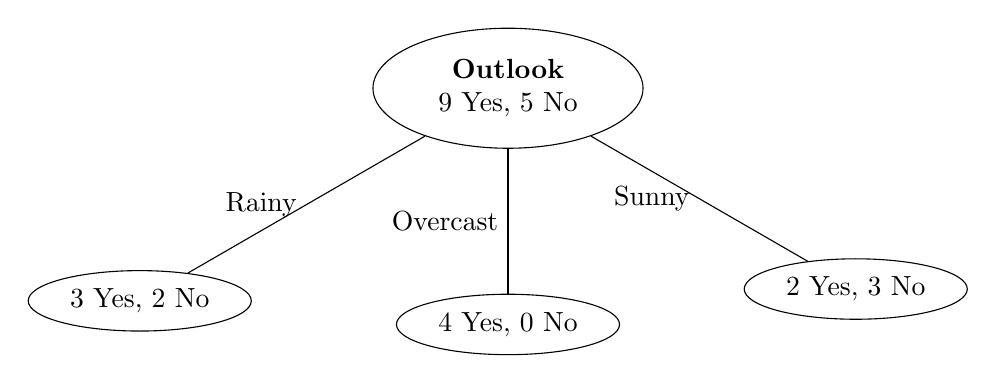
\begin{tikzpicture}[scale = 3] 
		
		\node (v0) at (0,0) [shape=ellipse, draw] {\begin{tabular}{c} \textbf{Outlook} \\ 9 Yes, 5 No\end{tabular}};
		\node (v1) at (210 : 1.80)[shape=ellipse, draw] {3 Yes, 2 No};
		\node (v2) at (270 : 1)[shape=ellipse, draw] {4 Yes, 0 No};
		\node (v3) at (330 : 1.70)[shape=ellipse, draw] {2 Yes, 3 No};
		
		\draw 
		(v0) -- (v1) node[draw=none,fill=none, midway, left] {Rainy};
		\draw
		(v0) -- (v2) node[draw=none,fill=none, midway, left] {Overcast};
		\draw
		(v0) -- (v3) node[draw=none,fill=none, midway, left] {Sunny};
	\end{tikzpicture}
\end{figure}


\FloatBarrier
\section{Gain Ratio}

Information gain favours attributes with many values over those with few values. If an attribute is highly branching, the splits generally tend to be small and heterogeneous causing the split entropies to be close to zero and thus resulting in very high information gain.

To avoid this difficulty, information gain is divided by a quantity called intrinsic information that is sensitive to highly branching attribues to give the gain ratio which is maximized instead.

\begin{align*}
	\textbf{IntrinsicInfo}(S, A) & = \sum_{i} \frac{|S_i|}{|S|} \times log_2(\frac{|S_i|}{|S|}) \\
	\textbf{GainRatio}(S, A)     & = \frac{\textbf{Gain}(S, A)}{\textbf{IntrinsicInfo}(S, A)}   
\end{align*}
\section{Refinements}

\subsection{Continuous Attributes} 

For a continuous attribute $\textbf{A}$, define a boolean attribute $\textbf{A}_c$ which is $True$ if $\textbf{A} < c$ and $False$ otherwise. To pick the optimal value of the threshold $c$ that maximizes the information gain, values of $\textbf{A}$ are sorted and candidate thresholds are generated midway of each consecutive pair.  


\begin{table}[h]
	\centering
	\begin{tabular}{c|cccccc}
		\toprule
		\textbf{Temperature} & 40 & 48 & 60  & 72  & 80  & 90 \\
		\midrule
		\textbf{PlayGolf}    & No & No & Yes & Yes & Yes & No \\
	\end{tabular}
\end{table}

Candidate thresholds and their information gain is computed as below. It is clear from the table below that $\textbf{Temperature} = 54$ is the optimal value for the threshold $c$.

\FloatBarrier
\begin{table}
	\centering
	\begin{tabular}{ |c|c|c|c| }
		\hline
		\textbf{Split} & \textbf{Yes} & \textbf{No} & \textbf{Gain}                     \\ 
		\hline
		$< 44$         & 0            & 1           & \multirow{2}{*}{0.191}            \\
		$>= 44$        & 3            & 2           &                                   \\
		\hline
		$< 54$         & 0            & 2           & \multirow{2}{*}{$\mathbf{0.459}$} \\
		$>= 54$        & 3            & 1           &                                   \\
		\hline
		$< 66$         & 1            & 2           & \multirow{2}{*}{0.082}            \\
		$>= 66$        & 2            & 1           &                                   \\
		\hline
		$< 76$         & 2            & 2           & \multirow{2}{*}{0}                \\
		$>= 76$        & 1            & 1           &                                   \\
		\hline
		$< 85$         & 3            & 2           & \multirow{2}{*}{0.191}            \\
		$>= 85$        & 0            & 1           &                                   \\
		\hline
	\end{tabular}
\end{table}

\FloatBarrier\clearpage

\subsection{Overfitting}

A hypothesis is said to overfit the training data if it performs very accurately on the training data but fares poorly on unseen test data. Two major approaches to avoid overfitting in decision tree learning are as follows:

\begin{itemize}
	\item Stop growing the tree before it starts to overfit.
	\item Grow tree fully but post prune it.
\end{itemize}

\subsubsection{Reduced Error Pruning}
Data is divided into training and validation sets. The training set is used to form the decision tree. Now, each decision node is considered for pruning. 

Pruning a decision tree consists of removing the subtree rooted at that node, making it a leaf node, and assigning it the most common classification of the training examples affiliated with that node. Nodes are removed only if the resulting tree performs no worse than the original tree over the validation set. 

Nodes are pruned iteratively, always choosing the node whose removal most increases the accuracy over the validation set. Pruning continues until further removal of nodes is harmful.

In case of limited data, the prospects of this pruning scheme are relatively dim. 

\subsubsection{Rule Post Pruning}

\begin{enumerate}
	\item Infer the decision tree from the training set allowing overfitting.
	\item Convert tree into equivalent set of rules by creating one rule per one path from root to a leaf node.
	\item Prune each rule by removing any preconditions that results in improving its estimated accuracy on the validation set. If a rule is of the form 
	      \begin{align*}
	      	  & IF\ (\textbf{Outlook}=Sunny)\wedge(\textbf{Humidity}=High) \\
	      	  & THEN\ \textbf{PlayGolf} = No                               
	      \end{align*}    
	      then $(\textbf{Outlook}=Sunny)$ and $(\textbf{Humidity}=High)$ are preconditions. 
	\item Sort the pruned rules by their estimated accuracy, and consider them in this sequence when classifying subsequent instances.
\end{enumerate}


\subsection{Missing Attributes Values}

\FloatBarrier\clearpage
\begin{figure}
	\centering
	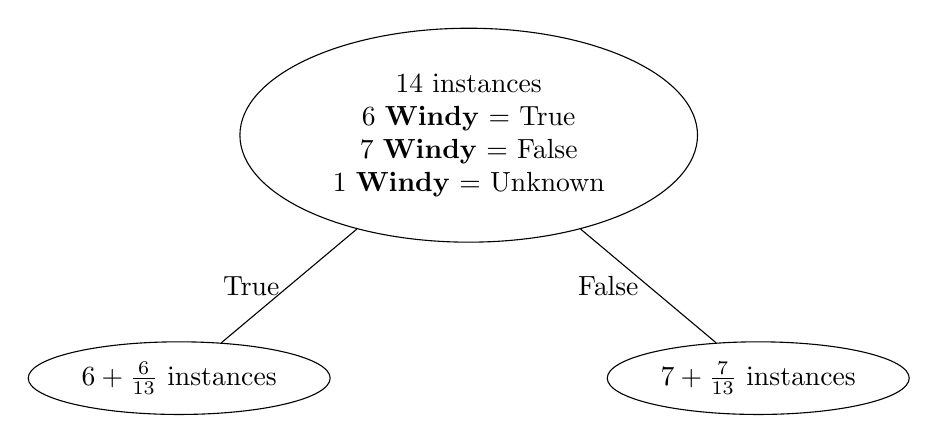
\begin{tikzpicture}[scale = 3] 
		
		\node (v0) at (0,0) [shape=ellipse, draw] {\begin{tabular}{c}
			14 instances \\ 
			6 \textbf{Windy} = True \\ 
			7 \textbf{Windy} = False \\
			1 \textbf{Windy} = Unknown \\
			\end{tabular}};
		\node (v1) at (220 : 1.60)[shape=ellipse, draw] {$6 + \frac{6}{13}$ instances};
		\node (v2) at (320 : 1.60)[shape=ellipse, draw] {$7 + \frac{7}{13}$ instances};
		
		\draw 
		(v0) -- (v1) node[draw=none,fill=none, midway, left] {True};
		\draw
		(v0) -- (v2) node[draw=none,fill=none, midway, left] {False};
	\end{tikzpicture}
\end{figure}



\subsection{Attribute With Differing Costs}
Instead of maximizing information gain ratio, a quantity like $\frac{f(\textbf{Gain}(S, A))}{g(\textbf{Cost}(S, A))}$ is maximized where $f$ and $g$ are chosen on a case by case basis.

\section{Comments}

\begin{itemize}
	\item Decision trees provide a practical method for concept learning and for learning other discrete-valued functions.
	\item A complete hyphothesis space is searched because the space of decision trees can represent any dicsrete-valued function defined over discrete valued instances. It therby avoids major difficulty associated with approaches that consider only restricted sets of hypothesis.
\end{itemize}

\end{document}